\documentclass{article}
\usepackage{graphicx} % Required for inserting images
\usepackage{float}
\usepackage[margin=1in]{geometry}
\usepackage{pgfplots}
\pgfplotsset{compat=1.18}


\title{Iscandar Revisited: Expansion to k=4 Theory For Running Debian}
\author{Andrew Jonathan Fine}
\date{November 2026}

\begin{document}

\maketitle

\begin{abstract}
This paper extends a deterministic memory allocator from radix depth k=3 to k=4 and tests the extension against a real operating system load. The k=3 design, published previously, allocates from a single cube of 32,768 sectors using an exact-fit bijection at radix 32. The k=4 extension composes cubes into beams under a rotary allocation rule, preserving the invariants of the k=3 theory: exact fit, bounded probes, and placement as a pure function of the request stream.\\

The load is a complete allocation census of an embedded Debian boot, captured from the kernel's own tracepoints: 812,106 allocations, with a standing set of 56,023 live objects at peak. That census rules out the k=3 design unconditionally, since one cube mints at most 32,768 handles. Replaying the identical stream through a four-cube beam at a 4 KiB grain, the k=4 system carries the entire load with no refusals and no free-path anomalies, peaking at 56,535 sectors against 56,599 pages granted by a binary buddy control in a matched arena. The 64-page difference is the buddy's power-of-two rounding, which exact fit holds instead as spendable free sectors. At a tighter 256 MiB arena the beam still refuses nothing, though the buddy's largest remaining fit exceeds the beam's, a structural consequence of the beam's cube boundaries. The claim is support by replay, with a potential DRAM savings, not in-kernel replacement.\\

A deterministic allocator can bear a general operating system's real load and gives nothing it cannot afford. Iscandar is able to conserve memory through implicit recognition of trapped and adjacent sectors.\\
\end{abstract}

\clearpage
\thispagestyle{empty}
\vspace*{\fill}
\begin{center}
\itshape To Jennifer: Everything. Always. Forever.
\end{center}
\vspace*{\fill}
\clearpage

\section{The Problem}

The prior paper~\cite{fine2026iscandar} established a deterministic allocator at radix depth k=3: a single cube of 32,768 sectors, exact fit by bijection, every request resolved by examining a fixed grid of counters in a fixed order, its costs bounded by ceilings that are theorems about the construction. Depth extension was named there as the route to scale. What the prior paper did not establish is whether the construction survives contact with a real operating system.\\

A cube mints at most 32,768 handles. A complete census of an embedded Debian boot, taken from the kernel's own tracepoints, shows a standing set of 56,023 live objects. No sector size cures a handle census: at k=3 the system cannot stand in for the operating system's allocator at any grain. The question is therefore not one of tuning but of structure.\\

We extend the construction to k=4, composing cubes into beams under a rotary rule, so the k=3 theory is preserved: exact fit, bounded probes, placement as a pure function of the request stream, and failure returned as a status. Then, we determine by replay if the extended system can bear the operating system's own measured load in the buddy allocator's place, judged in matched arenas by granted memory and by largest possible fit remaining (LPFR), at the end of the stream and at the instant of peak stress.

\section{The Extension to k=4}

\subsection{Coordinates}

The k=3 theory names every sector of a cube by a coordinate (plane, row, sector) under a bijection $B_3$ onto the displacements 0 to 32,767. The extension adds one field. A k=4 coordinate is a pair (c, x), where x is a k=3 coordinate and c, the cube index, ranges over the beam's cubes. The composed bijection is $B_4(c, x) = c \cdot 32768 + B_3(x)$. Nothing in the cube changes: its engines, its modes, and its proofs are the k=3 theory operating unchanged on x. The cube index is carried outermost, so projection back to k=3 is deletion of the leading field, and every k=4 name corresponds to exactly one sector of exactly one cube. The naming is a bijection because it is a composition of bijections.

\subsection{The Pointer}

Coordinates extend by adding a field; pointers extend by widening the packing. The k=4 pointer is a 64-bit word: one virtual bit, one reserved bit, a 30-bit start field composed of the 15-bit cube index over the 15-bit local start, and a 15-bit count field, the count stored reduced by one as at k=3. Forty-seven bits are in use. The seventeen spare bits sit in the start stack, above the cube field, where a further 15-bit start field would extend the same word to k=5; the count does not widen at any depth, because an allocation lives inside one cube by construction. A pointer is born virtual, minted only from a coordinate and a count; a pre-existing word enters only by adoption, under the k=3 discipline.

\subsection{The Beam}

A beam is a set of cubes, from 1 to 32, under a rotary order. Allocation first checks the beam's summed counters against the request, then asks the lead cube; on refusal it rotates and asks the next, and the first acceptance along the rotary order seats the allocation. Counts are checked before any commitment is made. At the moment of acceptance, and only then, the accepting cube's index is known, and the returned k=3 pointer is transformed: its coordinate acquires the cube index, and the pair is minted as a k=4 pointer. Deallocation is the allocation process read in reverse, as the bijection requires: the pointer decomposes into its cube index and its k=3 coordinate, the local pointer is unmarked in its own cube, and the beam's counter is decremented only on a success status.

\subsection{What Is Preserved}

The extension surrenders none of the k=3 guarantees. Fit remains exact: no request is rounded to a size class. Probes remain bounded: at most one probe per cube in the beam, each probe bounded by the k=3 ceilings. Placement remains a pure function of the request stream: the rotary order is fixed in advance, so the same stream produces the same pointers on every run. Live pointers never overlay, by construction, at either level. Failure is returned as a status, never as a crash or a silent substitution. And the arithmetic at every level is pure sector arithmetic: the sector size, the grain, is imposed only at the top, by whoever maps sectors to memory.

\section{Desk Check}

The theory section asserts; this section traces. We follow the code of \texttt{iscandar-k4} once, slowly, on a beam of four cubes, 131,072 sectors, and check at each step that the code does what the construction says it does. The wider design space of dynamic storage allocation is surveyed by Wilson et al.~\cite{wilson1995dynamic}.

\subsection{The Gates}

A request is refused by arithmetic before it is refused by search. The beam first checks itself:

\begin{verbatim}
if (self.sectors_supported - self.count_overall) < request:
  return
\end{verbatim}

and each cube, when asked, checks itself the same way inside \texttt{scan}, returning nothing without ever calling its engine if the request exceeds its own remaining count. Counts are checked before any commitment is made; a beam that cannot seat a request in sum never begins, and a cube that cannot seat it alone is never disturbed.

\subsection{Rotation and First Acceptance}

The allocate loop walks the rotary order: \texttt{scan} the lead cube; on an \texttt{MPUPointer} result, add the request to \texttt{count\_overall} and transform; on refusal, \texttt{rotate()} and ask the next, at most once per cube. First acceptance along the order seats the allocation, and the loop bound is the cardinality itself: the probes are bounded by the width of the beam.

\subsection{The Transform}

The accepting cube's index is known only at acceptance, and the code takes it there:

\begin{verbatim}
coordinate      = pointer.coordinate () # MPUPointer
beam_coordinate = BeamCoordinate (cube, coordinate.sector,
                                  coordinate.row, coordinate.plane)
return CPUPointer (beam_coordinate, pointer.count)
\end{verbatim}

Inside \texttt{CPUPointer}, the start field is computed as:
\begin{center}
    \texttt{coordinate.cube * Cube.SECTORS\_PER\_CUBE + local.displacement},\\
\end{center}
which is the composed bijection of the theory section written as one line of arithmetic: $B_4(c, x) = c \cdot 32768 + B_3(x)$, with the local displacement standing for $B_3(x)$.

\subsection{The Free Path}

Deallocation decomposes the pointer, reloads the local k=3 pointer by:
\begin{center}
\texttt{MPUPointer.load\_coordinate (coordinate.k3 (), pointer.count)}, 
\end{center}
and unmarks it in the cube named by the pointer's own cube field. The beam's counter is decremented only when the returned status is \texttt{GEAR\_SUCCESS}; the status itself is returned to the caller either way.

\subsection{A Worked Trace}

On a fresh \texttt{Beam(4)}: \texttt{allocate(100)} seats in cube 0 and returns the word \texttt{0x8000000000000063}: virtual bit set, start 0, stored count 99, the true count less one. \texttt{allocate(32768)} cannot seat in cube 0, which already holds 100 sectors and so fails its own per-cube gate; the beam rotates, cube 1 accepts, and the word is \texttt{0x8000000040007FFF}: start 32768, that is, cube 1 at local displacement 0, stored count 32767 for the whole cube. The beam's counter stands at 32,868. Freeing both pointers returns status 8, \texttt{GEAR\_SUCCESS}, both times, and the counter returns to exactly 0. Nothing was searched that arithmetic had already refused, nothing was committed before its count was checked, and the two words decode, field by field, to the coordinates the theory predicts.

\section{The Test}

\subsection{The Intention}

The test as first conceived was a test of the published system, at k=3. A stock embedded Debian would be built and booted, every allocation it made under its own buddy allocator would be recorded, and the resulting stream would be replayed through the k=3 engine to learn whether one cube could bear a real operating system's boot. The expectation that the attempt was reasonable came from the uncrating: the original drive suggested an initramfs on the order of 128K under the buddy system, a modest load to set against 32,768 handles.\\

The apparatus was arranged to keep the load honest. ELBE was installed from its released packages and pinned, and the test image, Fubuki, was built from our project description alone: the tool is the stock car, and we authored no part of the Debian it builds. The image runs under QEMU on a serial console, with no video, and the boot ends at the login prompt: the prompt is the boundary of the experiment, and everything before it is the load. Recording is by the kernel's own built-in tracepoints at the kmalloc level. No source was marked up, patched, or otherwise persuaded: the list of allocations is the list the buddy system itself produced, in the order it produced it.

\subsection{The Reality}

The first boots failed, and they failed on the rig, not on Iscandar. At 128 MiB the image died in the initramfs unpack, stock Debian under its own allocator, before our system had any part in the proceedings, and the trace buffer sizing took attempts of its own. The configuration that boots honestly is 512 MiB, and it is at 512 MiB that the capture of record was taken: 1,650,424 events, the header counts equal, zero overruns, resolving to 812,106 allocations and their frees.\\

The census then answered the original question before any replay could. At peak, the boot holds 56,023 live objects. One cube mints at most 32,768 handles, at any sector size: the shortage is in handles, not in bytes, and no grain cures it. The k=3 system cannot stand in for this load, unconditionally. The test was therefore rebuilt around the k=4 extension, for both of its legs alike: the buddy control replayed over the same stream in matched arenas, and the experiment proper run through the beam.\\

Let the reframing be read correctly. It is not an indictment of Iscandar. The panics belonged to the test configuration, and the handle shortage marks the boundary of the domain the k=3 theory was published for: bounded loads, censused in advance. A general operating system boot stands outside that domain by census, and a design is not indicted by meeting a load it never claimed. What the measurement took from k=3, it gave to the question: not whether the published system suffices for Debian, but whether its extension does.\\

The test data was generated on the author's laptop. Fubuki was built with ELBE 15.9 from Debian 13 (trixie) and booted under QEMU on that machine; the trace used in this test is the kernel's own record of that boot.

\section{The Control}

The control is the incumbent, given the same load and every advantage of the matched configuration. The identical stream is replayed through a binary buddy allocator~\cite{knuth1997art1} over an arena of 131,072 pages of 4 KiB, the 512 MiB of the machine under test. Each request is first reduced to pages at the stated grain, then granted the smallest power of two page count that covers it, placed at the lowest address that fits, split and coalesced by the buddy rules. The model's list discipline is simpler than the kernel's; its geometry is the kernel's: powers of two, one arena, history-dependent placement. It is the geometry that is under test, and the geometry is not a straw man.\\

The harness discipline is shared with the experiment, and is stated here once. When the stream allocates through a pointer the driver still holds live, the old pointer is freed first and counted as an inferred free: 1,736 such events, the trace's own bookkeeping made explicit rather than silently orphaned. Frees of unknown pointers are counted and skipped: 83,968, the allocations for which the trace window holds no birth. Occupancy and largest possible fit remaining are sampled on the same schedule for both systems.\\

The control's calibration is exact. Its live set peaks at 56,023 objects occupying 56,535 pages of pure demand, reproducing the census of The Test to the page. What it grants is more than the demand, by the buddy's own arithmetic: peak granted 56,599 pages, 221.09 MiB, the excess of 64 pages being the power-of-two rounding of the live set's requests, a quantity fixed by the size distribution alone. At the end of the stream it grants 56,596 pages and refuses nothing at any point. Its largest possible fit remaining never falls below 65,536 pages: in an arena this size, against this load, a block of 256 MiB is grantable at every sampled instant.\\

That is the mark. The control carries the boot at a cost of 56,599 pages granted, with a vast contiguous remainder, in the arena the machine actually has. The experiment is asked to meet it in the same arena, at the same grain, under the same discipline.

\section{The Experiment}

The experiment is the same stream, the same discipline, and the same arena, with the beam in the buddy's place. A beam of four cubes stands over 131,072 sectors of 4 KiB, the 512 MiB of the machine under test. Each request is reduced to sectors on its requested bytes alone, and the driver keeps the live set itself, sampling every thousand events. Largest possible fit remaining is read off the engines' own sector stores, as the largest contiguous free run inside any one cube: by construction it cannot exceed one cube, 32,768 sectors, and that ceiling is part of the measurement, not an apology for it.\\

The beam carries the whole stream. Of 1,650,424 events it refuses nothing and reports no free-path anomaly: the 1,736 inferred frees and 83,968 unknown frees arise under the shared harness discipline stated in The Control. Its live set peaks at 56,535 sectors in 56,023 objects, reproducing the census of The Test exactly, by an independent route. At the end of the stream it holds 56,532 sectors in 56,020 objects. Its largest possible fit remaining never falls below 32,768 sectors: a whole cube is grantable at every sampled instant.

\section{The Comparison}

Against the control, the difference is one number with two readings. The control granted 56,599 pages at peak; the beam's demand at peak is 56,535 sectors, and under exact fit demand and grant are the same number. The 64 pages between them, 256 KiB, are the buddy's power-of-two rounding: memory the buddy locks inside its own grants, welded to the blocks that hold it, and the beam holds instead as free sectors, which answer requests. The difference is small at this arena and it is also absolute: there is a band of arena sizes 64 pages wide in which the two systems return different verdicts on this identical load, an arena of 56,560 pages sufficing for the beam and not for the control.\\

On contiguity the honest report is that this arena stresses neither system. The beam's largest possible fit remaining never falls below 32,768 sectors, and the control's never falls below 65,536 pages. Both floors are set by the arena's generosity rather than by either allocator's character under pressure, and this paper does not pretend otherwise: what the matched configuration establishes is parity on the incumbent's own axes, granted totals and remainder alike, from a system whose placements are a pure function of the stream.\\

Two figures accompany this section: occupancy over the stream for both systems, and largest possible fit remaining over the stream for both systems, The Real Debian Numbers:  Macroscopically identical, microscopically different, and the microscopic difference is the contribution.\\ 




\begin{figure}[H]
\centering
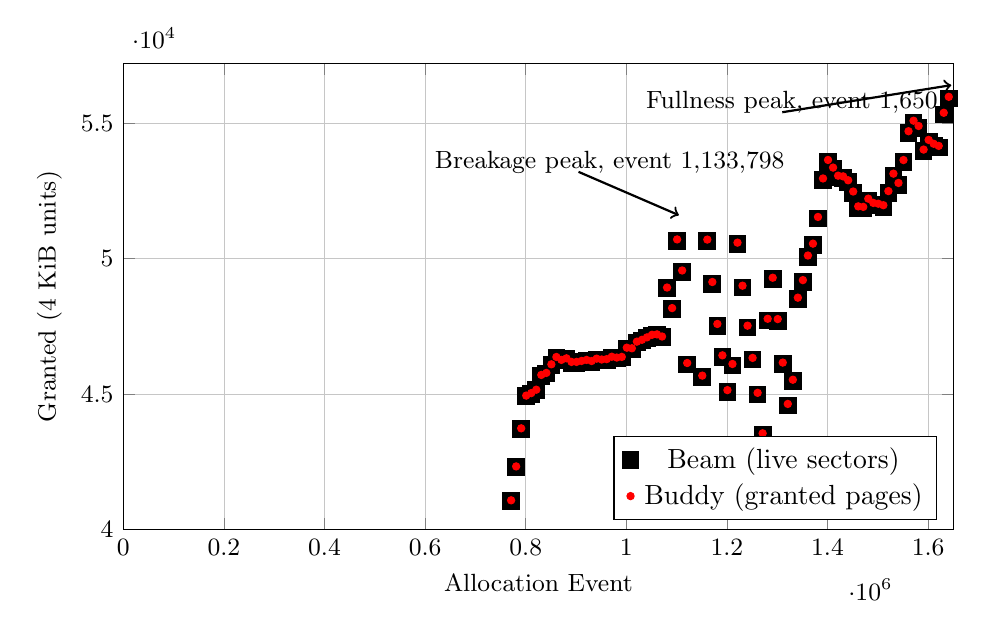
\begin{tikzpicture}
\begin{axis}[
  width=\textwidth, height=7.5cm,
  xlabel={Allocation Event},
  ylabel={Granted (4 KiB units)},
  xmin=0, xmax=1650424, ymin=40000, ymax=57200,
  legend style={at={(0.98,0.02)}, anchor=south east},
  grid=both, grid style={line width=.1pt, draw=gray!20},
  major grid style={line width=.2pt, draw=gray!45},
  tick label style={font=\small},
  label style={font=\small},
]
\addplot[black, only marks, mark=square*, mark size=3] coordinates {
(1000,888) (11000,5185) (21000,6297) (31000,7723) (41000,8320) (51000,15194) (61000,17872) (71000,20019)
(81000,20278) (91000,20281) (101000,20345) (111000,20354) (121000,20430) (131000,20464) (141000,20458) (151000,20526)
(161000,20548) (171000,20586) (181000,20580) (191000,20624) (201000,20640) (211000,20722) (221000,20720) (231000,20758)
(241000,20732) (251000,20744) (261000,20826) (271000,20772) (281000,20868) (291000,20824) (301000,20822) (311000,20866)
(321000,20920) (331000,20894) (341000,20176) (351000,20256) (361000,20318) (371000,20362) (381000,20414) (391000,20468)
(401000,20518) (411000,20520) (421000,20546) (431000,20610) (441000,20596) (451000,20640) (461000,20652) (471000,20690)
(481000,20734) (491000,20738) (501000,20760) (511000,20762) (521000,20802) (531000,20794) (541000,20894) (551000,20834)
(561000,20858) (571000,20876) (581000,20900) (591000,20994) (601000,21026) (611000,23122) (621000,27229) (631000,29328)
(641000,30032) (651000,30125) (661000,30686) (671000,30998) (681000,31394) (691000,33641) (701000,35187) (711000,36094)
(721000,36819) (731000,37344) (741000,37760) (751000,38256) (761000,39129) (771000,41061) (781000,42311) (791000,43717)
(801000,44921) (811000,45013) (821000,45138) (831000,45678) (841000,45752) (851000,46069) (861000,46339) (871000,46232)
(881000,46290) (891000,46157) (901000,46157) (911000,46193) (921000,46231) (931000,46191) (941000,46278) (951000,46247)
(961000,46261) (971000,46349) (981000,46319) (991000,46343) (1001000,46682) (1011000,46660) (1021000,46904) (1031000,46972)
(1041000,47062) (1051000,47156) (1061000,47172) (1071000,47094) (1081000,48900) (1091000,48142) (1101000,50647) (1111000,49501)
(1121000,46086) (1131000,42956) (1141000,42193) (1151000,45619) (1161000,50637) (1171000,49071) (1181000,47523) (1191000,46365)
(1201000,45081) (1211000,46049) (1221000,50524) (1231000,48935) (1241000,47459) (1251000,46270) (1261000,44981) (1271000,43490)
(1281000,47718) (1291000,49233) (1301000,47707) (1311000,46101) (1321000,44575) (1331000,45468) (1341000,48497) (1351000,49145)
(1361000,50052) (1371000,50490) (1381000,51476) (1391000,52892) (1401000,53575) (1411000,53293) (1421000,52994) (1431000,52969)
(1441000,52825) (1451000,52410) (1461000,51862) (1471000,51843) (1481000,52146) (1491000,51990) (1501000,51960) (1511000,51905)
(1521000,52426) (1531000,53069) (1541000,52726) (1551000,53571) (1561000,54636) (1571000,55023) (1581000,54829) (1591000,53958)
(1601000,54315) (1611000,54172) (1621000,54094) (1631000,55316) (1641000,55905)
};
\addlegendentry{Beam (live sectors)}
\addplot[red, only marks, mark=*, mark size=1.3] coordinates {
(1000,891) (11000,5188) (21000,6300) (31000,7726) (41000,8323) (51000,15210) (61000,17888) (71000,20035)
(81000,20293) (91000,20296) (101000,20360) (111000,20369) (121000,20445) (131000,20479) (141000,20473) (151000,20541)
(161000,20563) (171000,20601) (181000,20595) (191000,20639) (201000,20655) (211000,20737) (221000,20735) (231000,20773)
(241000,20747) (251000,20759) (261000,20841) (271000,20787) (281000,20883) (291000,20839) (301000,20837) (311000,20881)
(321000,20935) (331000,20909) (341000,20191) (351000,20271) (361000,20333) (371000,20377) (381000,20429) (391000,20483)
(401000,20533) (411000,20535) (421000,20561) (431000,20625) (441000,20611) (451000,20655) (461000,20667) (471000,20705)
(481000,20749) (491000,20753) (501000,20775) (511000,20777) (521000,20817) (531000,20809) (541000,20909) (551000,20849)
(561000,20873) (571000,20891) (581000,20915) (591000,21009) (601000,21041) (611000,23137) (621000,27244) (631000,29343)
(641000,30047) (651000,30140) (661000,30701) (671000,31013) (681000,31409) (691000,33656) (701000,35202) (711000,36109)
(721000,36834) (731000,37359) (741000,37775) (751000,38271) (761000,39144) (771000,41077) (781000,42328) (791000,43734)
(801000,44942) (811000,45034) (821000,45159) (831000,45705) (841000,45779) (851000,46097) (861000,46367) (871000,46260)
(881000,46318) (891000,46185) (901000,46185) (911000,46221) (921000,46259) (931000,46218) (941000,46305) (951000,46274)
(961000,46288) (971000,46376) (981000,46346) (991000,46370) (1001000,46710) (1011000,46688) (1021000,46933) (1031000,47001)
(1041000,47091) (1051000,47185) (1061000,47201) (1071000,47123) (1081000,48930) (1091000,48172) (1101000,50706) (1111000,49560)
(1121000,46145) (1131000,43015) (1141000,42252) (1151000,45679) (1161000,50700) (1171000,49134) (1181000,47586) (1191000,46428)
(1201000,45144) (1211000,46109) (1221000,50587) (1231000,48998) (1241000,47522) (1251000,46333) (1261000,45044) (1271000,43550)
(1281000,47777) (1291000,49292) (1301000,47766) (1311000,46160) (1321000,44634) (1331000,45527) (1341000,48556) (1351000,49204)
(1361000,50111) (1371000,50550) (1381000,51535) (1391000,52956) (1401000,53639) (1411000,53357) (1421000,53058) (1431000,53033)
(1441000,52889) (1451000,52474) (1461000,51926) (1471000,51907) (1481000,52210) (1491000,52054) (1501000,52024) (1511000,51969)
(1521000,52490) (1531000,53133) (1541000,52790) (1551000,53635) (1561000,54700) (1571000,55087) (1581000,54893) (1591000,54022)
(1601000,54379) (1611000,54236) (1621000,54158) (1631000,55380) (1641000,55969)
};
\addlegendentry{Buddy (granted pages)}
\node[anchor=south west, font=\small] at (axis cs:1020000,55000) {Fullness peak, event 1,650,412};
\draw[->, thick] (axis cs:1310000,55400) -- (axis cs:1646000,56400);
\node[anchor=south west, font=\small] at (axis cs:600000,52800) {Breakage peak, event 1,133,798};
\draw[->, thick] (axis cs:905000,53200) -- (axis cs:1104500,51600);
\end{axis}
\end{tikzpicture}
\caption{Occupancy over the stream, vertical axis magnified, every tenth sample: black squares, Iscandar; red rounds, buddy. The buddy rides above the beam by at most 64 pages. The arrows mark the two stress peaks examined in the Stress Testing section. The fullness peak, event 1,650,412, is where granted occupancy is maximal: the maximum stress maps are taken there. The breakage arrow marks the last sample before the fall: the breakage peak itself, event 1,133,798, lies at the bottom of the descent that follows, where the buddy's free space stood most fragmented in the halved arena: 24,543 pages free, its largest fit at its floor of 8,192 pages.}
\label{fig:occupancy}
\end{figure}

% Figure 2: Largest Possible Fit Remaining (LPFR), pgfplots, data inline.
% Verified 2026-11-05 from the replay series: in series-honest.csv the beam's
% lpfr_sectors is 32768 at every one of the 1650 samples (events 1000..1650000),
% and in series-buddy.csv the buddy's lpfr_pages is 65536 at every sample.
% The lines are therefore exactly flat, so two endpoints per line are the
% complete data, not a downsampling. No CSV files needed in the project.
% Preamble needs: \usepackage{pgfplots} and \pgfplotsset{compat=1.18}
\begin{figure}[H]
\centering
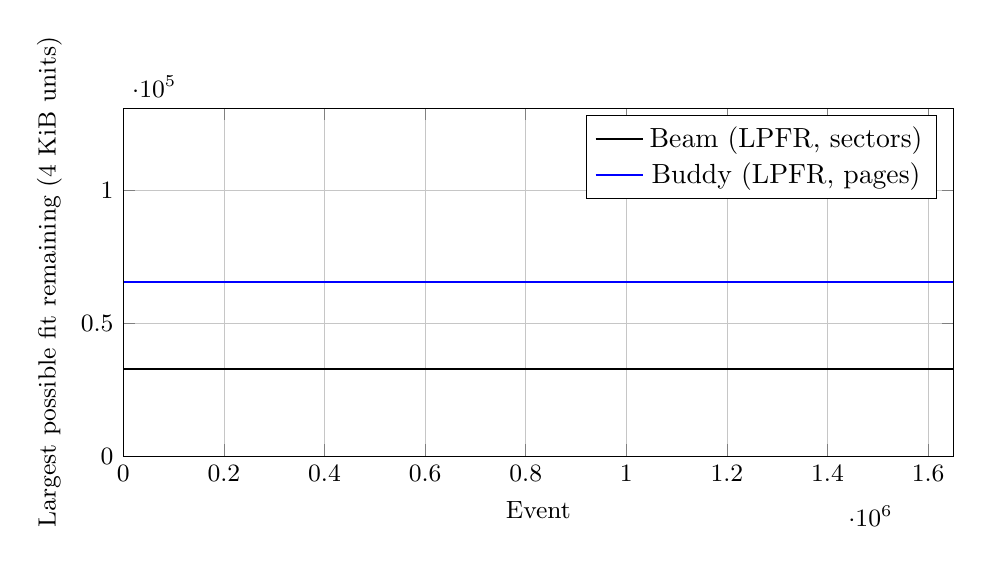
\begin{tikzpicture}
\begin{axis}[
width=\textwidth, height=6cm,
xlabel={Event},
ylabel={Largest possible fit remaining (4 KiB units)},
xmin=0, xmax=1650424, ymin=0, ymax=131072,
legend style={at={(0.98,0.98)}, anchor=north east},
grid=both, grid style={line width=.1pt, draw=gray!20},
major grid style={line width=.2pt, draw=gray!45},
tick label style={font=\small},
label style={font=\small},
]
\addplot[black, thick] coordinates {
(1000,32768) (1650000,32768)
};
\addlegendentry{Beam (LPFR, sectors)}
\addplot[blue, thick] coordinates {
(1000,65536) (1650000,65536)
};
\addlegendentry{Buddy (LPFR, pages)}
\end{axis}
\end{tikzpicture}
\caption{Largest possible fit remaining over the stream, in 4 KiB units. The arenas are matched at 131,072 units each, 512 MiB: four cubes for the beam, one span of pages for the buddy. Both lines are flat at every sample. The beam's line stands at 32,768 sectors, one whole cube, because no fit can cross a cube wall and at least one cube stands empty throughout. The buddy's line stands at 65,536 pages, half its arena in a single block. At this arena, neither system is stressed on contiguity.}
\label{fig:lpfr}
\end{figure}

A note on where the maximum falls. In both systems the instant of maximum stress arrives twelve events before the end of the stream, at event 1,650,412, and this is a property of the load, not of either allocator. A boot accumulates: most of what the kernel allocates is resident state, taken as its phase arrives and not freed before the prompt. Occupancy therefore climbs as a staircase: a long plateau near 20,500 live sectors, another near 46,300, then the final rise as the last services and the login stack come up. The churn rides on the staircase, its median lifetime seven microseconds, too small to outbid the accumulated set for the peak. And the end of the stream is the experiment's boundary, the login prompt, not a shutdown: the frees that would draw occupancy down were never recorded. Both systems are therefore judged at nearly the same instant for a structural reason: the machine finishes filling itself just before the trace closes, and the last dozen events, a few init paths freeing their scratch on the way out, lower the granted total by three pages, from 56,599 to 56,596.\\

Set side by side at the two instants of the fall, the systems trade the same ground in opposite shapes. At the crest the control stands nearly solid, 51,767 pages granted with its largest fit already at its floor of 8,192, while the beam holds 51,708 live sectors with its lead cube's largest run down to 15 sectors and its reserve cube offering 5,920. At the bottom the control holds 24,543 free pages but can offer no fit above 8,192, with 10,953 of those pages stranded in holes inside its span; the beam holds 24,602 free sectors, 59 more, its largest fit 5,377 in its emptier cube, and every free sector spendable at its own size, freed sectors having returned to service with no coalescing step between a free and its reuse. Neither system refused a request at either instant. The difference is in what their free memory is: the control's is a quantity, the beam's is an inventory.

\section{Stress Testing}

The matched configuration of The Control and The Experiment, a 512 MiB arena, stresses neither system: granted totals peak near 56,600 units of 131,072, and the largest possible fit remaining never falls below half the arena. To see the systems under pressure the arena is halved, to 256 MiB, and the stream is stopped at the instant of maximum stress: peak granted occupancy, which in both systems falls at event 1,650,412 of 1,650,424, twelve events before the end.

\subsection{Buddy System}

Within the control's run, the telling episode is a fall. Occupancy climbs its staircase to a crest at event 1,106,000, where 51,767 pages stand granted in the halved arena, then falls away as a phase of the boot lets its population die, bottoming at event 1,133,798 with 40,993 pages granted. Figure~\ref{fig:buddycrest} maps the top of the crest, Figure~\ref{fig:buddybottom} the bottom, and Figure~\ref{fig:buddyfinal} the end of the stream in the halved arena, where 56,596 pages stand granted of 65,536.\\

\begin{figure}[H]
\centering
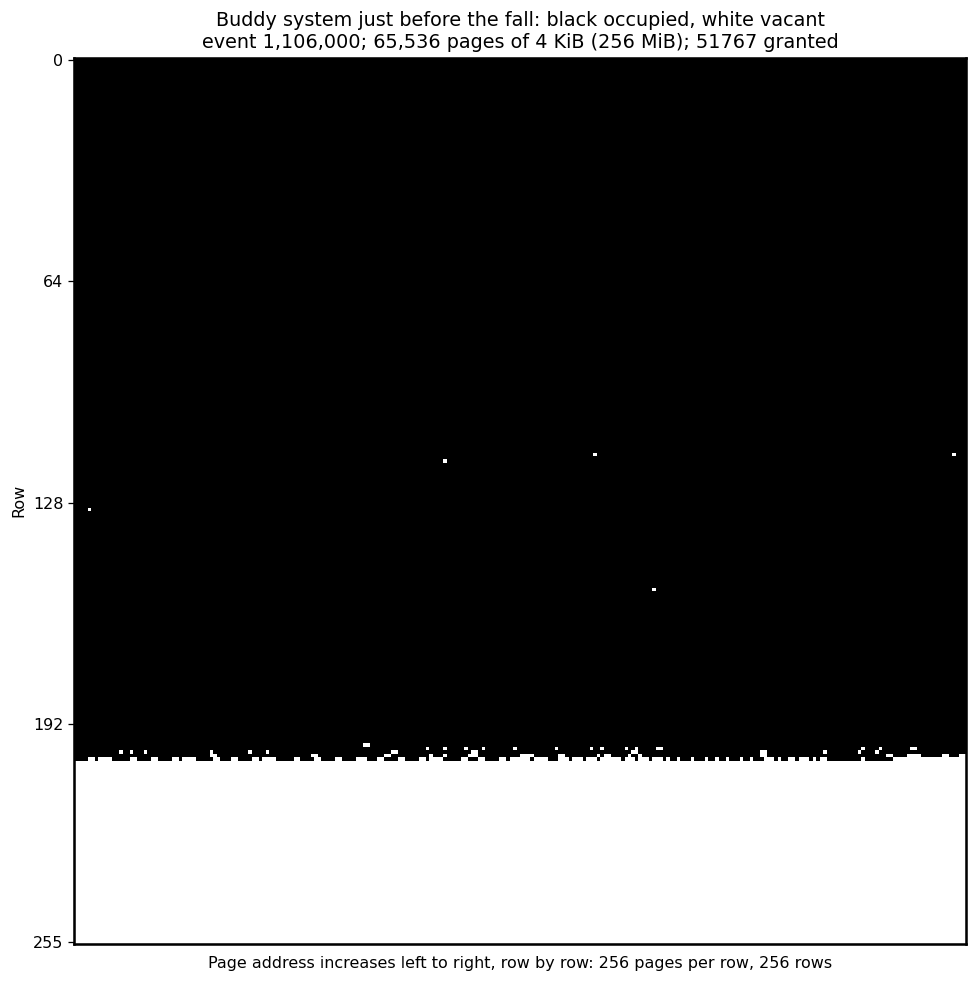
\includegraphics[width=\textwidth]{buddy-1106000-map.png}
\caption{The buddy system at the top of the crest, 256 MiB arena, event 1,106,000. Black is occupied, white is vacant; each cell is one 4 KiB page. 51,767 pages are granted, and 180 vacant pages already stand inside the occupied span; the largest possible fit remaining is already at its floor of 8,192 pages.}
\label{fig:buddycrest}
\end{figure}

\begin{figure}[H]
\centering
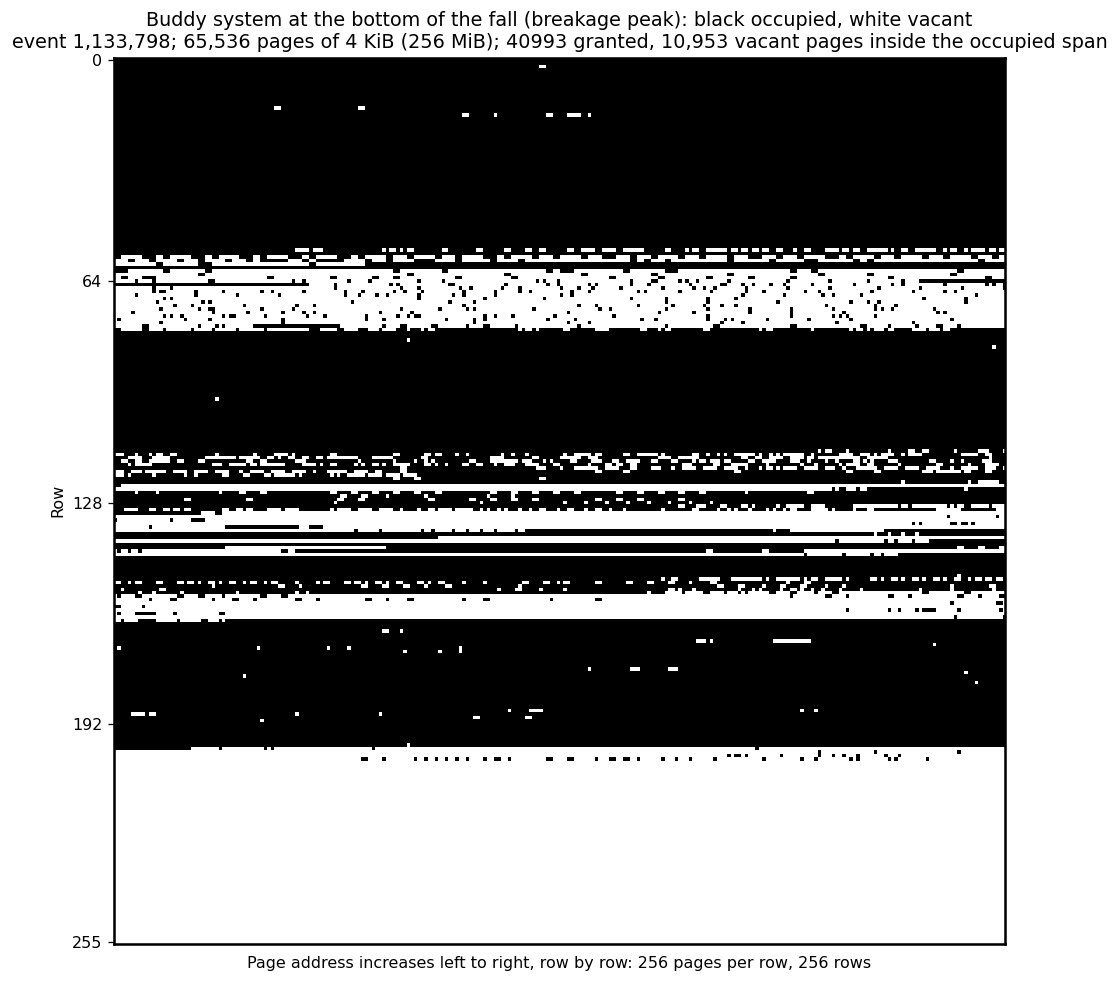
\includegraphics[width=\textwidth]{buddy-1133798-map.png}
\caption{The buddy system at the bottom of the fall, the breakage peak, 256 MiB arena, event 1,133,798. Black is occupied, white is vacant; each cell is one 4 KiB page. Granted has fallen to 40,993, and the occupied span is hollow: 10,953 vacant pages in 1,108 separate holes, the largest hole 465 pages, with 24,543 pages free in all and no single fit larger than 8,192.}
\label{fig:buddybottom}
\end{figure}

\begin{figure}[H]
\centering
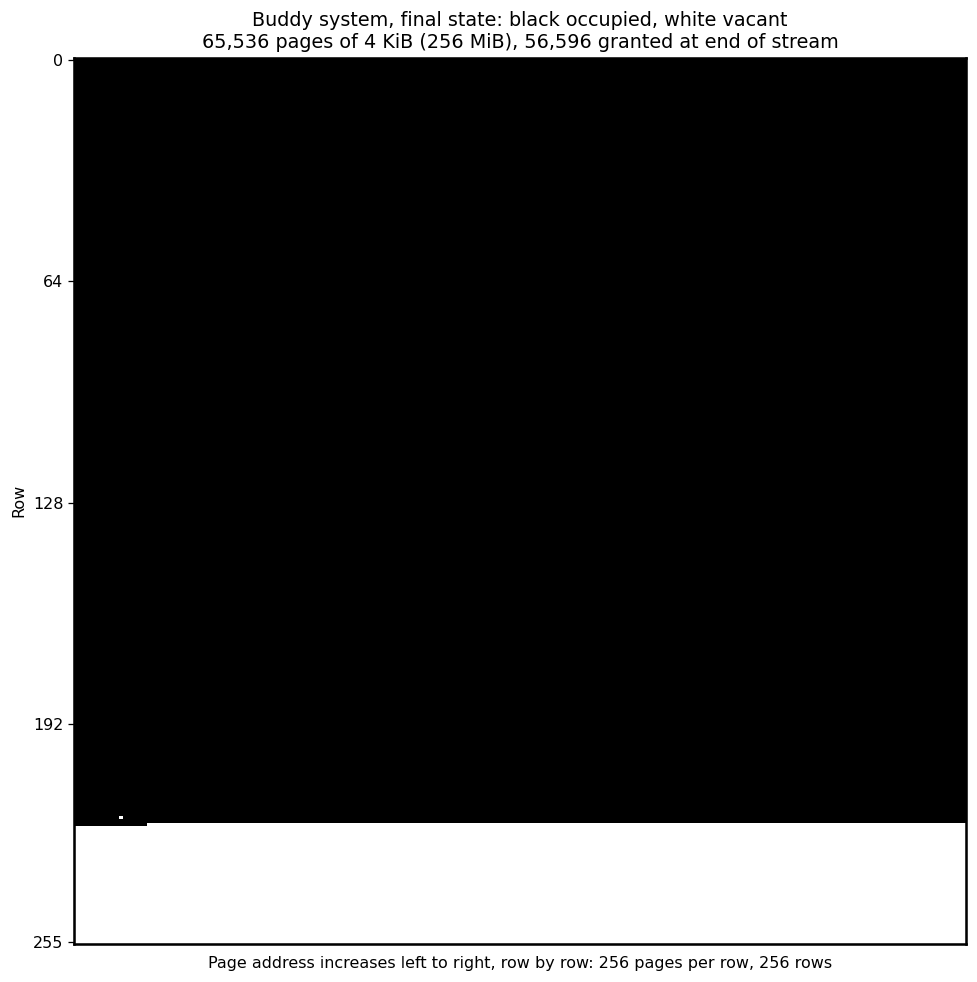
\includegraphics[width=\textwidth]{buddy-final-state-map.png}
\caption{The buddy system at the end of the stream, 256 MiB arena. Black is occupied, white is vacant; each cell is one 4 KiB page. Inside the occupied span, which runs from page 0 to page 56,596, there is exactly one vacant page.}
\label{fig:buddyfinal}
\end{figure}

Read in order, the buddy system maps are the biography of the free space under first, best fit. At the crest the span is nearly solid: the climb has packed it, and only 180 holes stand inside it, though the largest fit is already at its floor. The fall hollows it: freeing punches a hole wherever a dying object lived, coalescing closes only the holes whose buddies are also free, and at the bottom the span holds 10,953 vacant pages it cannot offer as one piece. Then the climb out refills it from the bottom, first fit taking the lowest holes first, until at the end of the stream the span is solid again but for a single page. This shows from classic buddy system algorithm under first, best fit~\cite{robson1977worstcase}: each allocation takes the lowest-addressed free block of the smallest sufficient order and splits it down, and each free coalesces with its buddy while the buddy is free. The system never refused a request on this load. But at the bottom of the fall it would have refused any request above 8,192 pages, with 24,543 pages standing free: coping in totals, barely coping in shape.

\subsection{Beam}

The beam is shown at the same two instants, in the same halved arena of two cubes. Figure~\ref{fig:beamcrest} maps the top of the crest, event 1,106,000, where the beam holds 51,708 live sectors in 51,241 objects and cube 0, which has taken the climb, stands 97.5 percent full. Figure~\ref{fig:beambottom} maps the bottom of the fall, event 1,133,798, where the beam holds 40,934 live sectors in 40,480 objects. Figure~\ref{fig:beamfinal} maps the end of the stream in the halved arena, where 56,532 sectors stand live and 9,004 are free.

\begin{figure}[H]
\centering
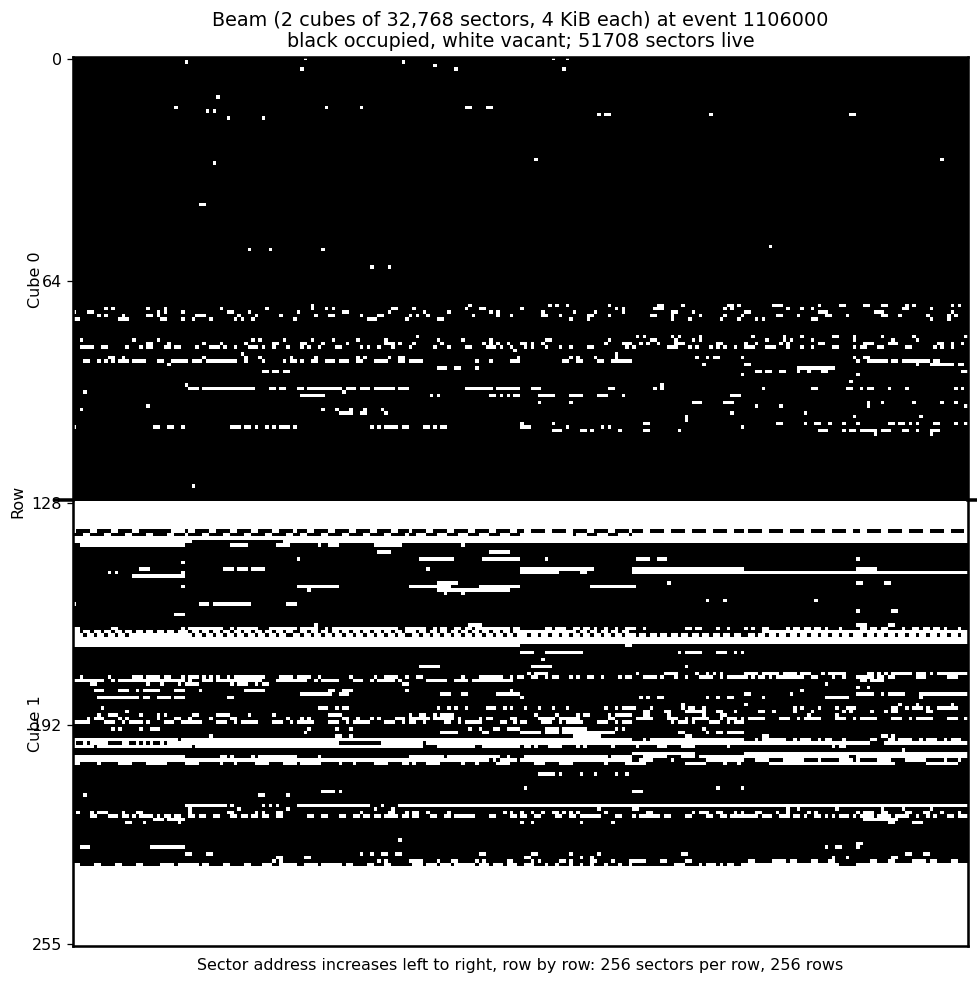
\includegraphics[width=\textwidth]{beam-1106000-map.png}
\caption{The beam at the top of the crest, two cubes, 256 MiB arena, event 1,106,000. Black is occupied, white is vacant; each cell is one 4 KiB sector. Cube 0 stands 97.5 percent full: 809 sectors free in 503 runs, its largest run 15. Cube 1 holds the reserve: 13,019 sectors free, its largest run 5,920.}
\label{fig:beamcrest}
\end{figure}

\begin{figure}[H]
\centering
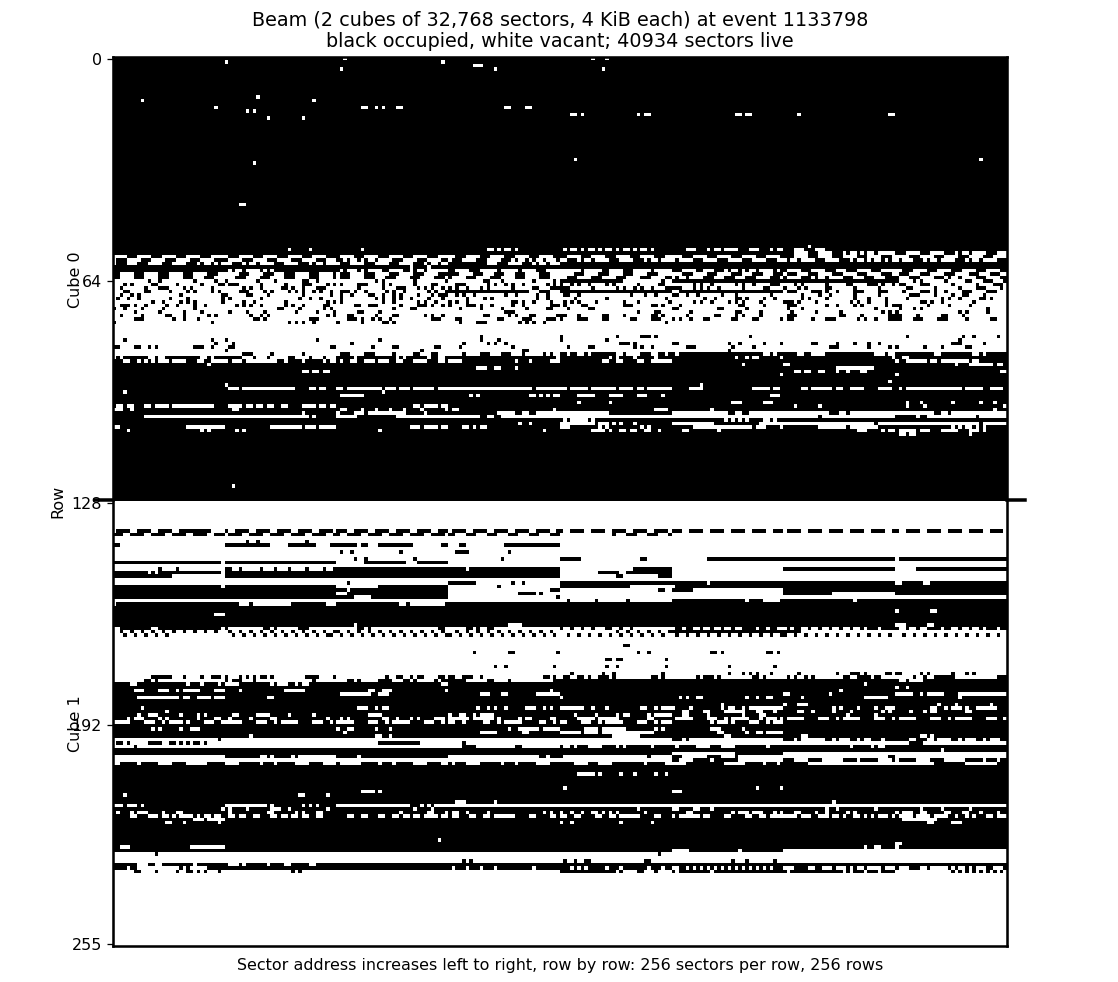
\includegraphics[width=\textwidth]{beam-1133798-map.png}
\caption{The beam at the bottom of the fall, two cubes, 256 MiB arena, event 1,133,798. Black is occupied, white is vacant; each cell is one 4 KiB sector. 24,602 sectors stand free. Cube 0's largest run stands restored at 970 sectors, and cube 1's at 5,377.}
\label{fig:beambottom}
\end{figure}

\begin{figure}[H]
\centering
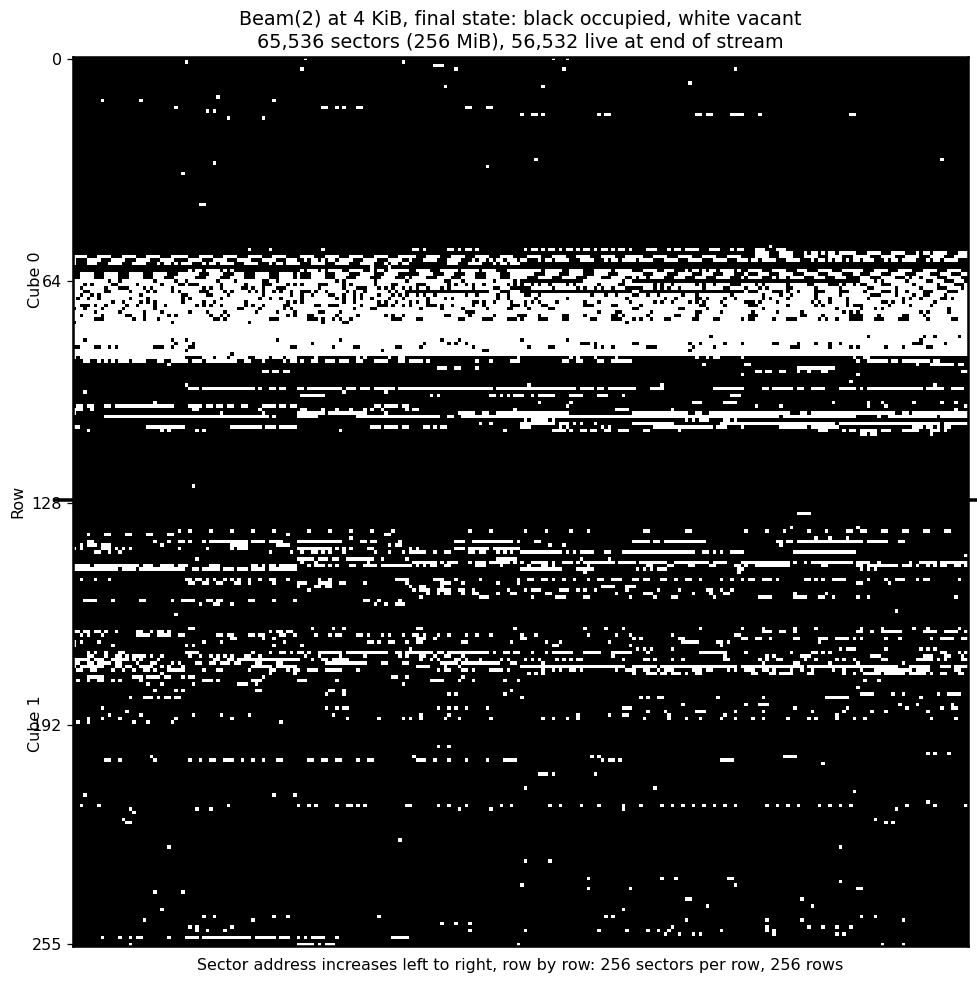
\includegraphics[width=\textwidth]{beam-final-state-map.png}
\caption{The beam at the end of the stream, two cubes, 256 MiB arena. Black is occupied, white is vacant; each cell is one 4 KiB sector. 56,532 sectors stand live and 9,004 free, in a fine speckle of runs across both cubes, every vacant sector reusable.}
\label{fig:beamfinal}
\end{figure}

\section{Conclusion}

The beam's maps look scattered at every instant, and the scatter is the design rather than a symptom. Because placement is exact and guided by the oracles, a freed sector is indistinguishable from one never granted: there is no coalescing step, no buddy that must also die before a free sector can be spent again. The transfer of free sectors back into service is nearly instant. Between the crest and the bottom, 10,774 sectors passed from live to free, and every one of them was available to the very next request at its own size. The buddy system's gathered pool is bought with work on every free, its merge cascade run in anticipation of large usages that may never arrive.\\

The beam does no such work and anticipates nothing: under high fragmentation it spends the runs that stand, at the sizes they stand. The cost of the design is the one the maps also show: a fit is walled inside a single cube, so the beam's largest single fit is whatever the emptiest cube can offer whole. What the beam keeps, at every instant, is the whole of its free space in spendable form.

\section{Questions \& Answers}

\textbf{How are free adjacent sectors joined?}
They are not joined through a process. They are recognized as adjacent during an O(1) search via the oracles. There is no coalescing pass and nothing is maintained on the free path: contiguity is a fact the tables already know, not a structure the allocator builds. The details are in the author's first paper, Project Iscandar~\cite{fine2026iscandar}.\\

\textbf{The arena stood mostly empty, so what does the test prove?}
How the arena stood empty matters more than that it stood empty. Two systems built for two entirely different problem classes behaved identically under the same load, with a slight nod toward Iscandar on overall savings: 56,535 sectors against 56,599 pages at the peak.\\

\textbf{Is a mathematical model enough, without running the allocator in a live system?}
Mathematical modelling to stringent enough parameters is sufficient for this test. The next step is to directly patch Fubuki's operating system, and this is left as an exercise for the hacker.\\

\textbf{Is this not a special-purpose allocator tested outside its element?}
Iscandar is designed to allocate from a closed memory system. That it can provide working memory under conventional conditions at all is unusual.\\

\textbf{Are the oracle tables not too heavy to be practical?}
The oracles need only be generated once per microprocessor, and they can be shared between Cubes, the fundamental large scale allocator unit. One generated set serves every cube in the system; it is not generated per cube, and the whole of it fits on a single thumb drive.

\section*{Acknowledgements}

The author is increasingly disabled from diabetes. At his direction, Muse translated his theorems into Python code, ran tests for him, and created the graphs in this paper from those tests.

\bibliographystyle{plain}
\bibliography{paper-2-refs}
\end{document}
